\documentclass[a4paper, top=10mm]{article}
%for writing from the top
\usepackage{fullpage}
%for math
\usepackage{amsmath}
\usepackage{mathrsfs}
\usepackage{amsthm}
%for images
\usepackage{graphicx}
%for color
\usepackage{xcolor}
%for title
\title{\textbf{\huge{Christmas Balls}}}
\author{Enigma n\textsuperscript{o}8}
\date{14\textsuperscript{th} December 2023}

\newtheorem*{hint}{Hint}

\addtolength{\voffset}{-2cm}
\addtolength{\textheight}{5cm}


\begin{document}
	\maketitle
	
	You are manufacturing magical Christmas decorations.
	All of them  are $n$-dimensional balls (hyper-balls, if you prefer), and they all have a radius of one.
	However, the decorations are magical, and may live in any dimension.
	You want to know what is the minimal and maximal volume of the decorations.
	
	\begin{center}
		
\includegraphics[width=0.3\linewidth]{08dimension1.png}	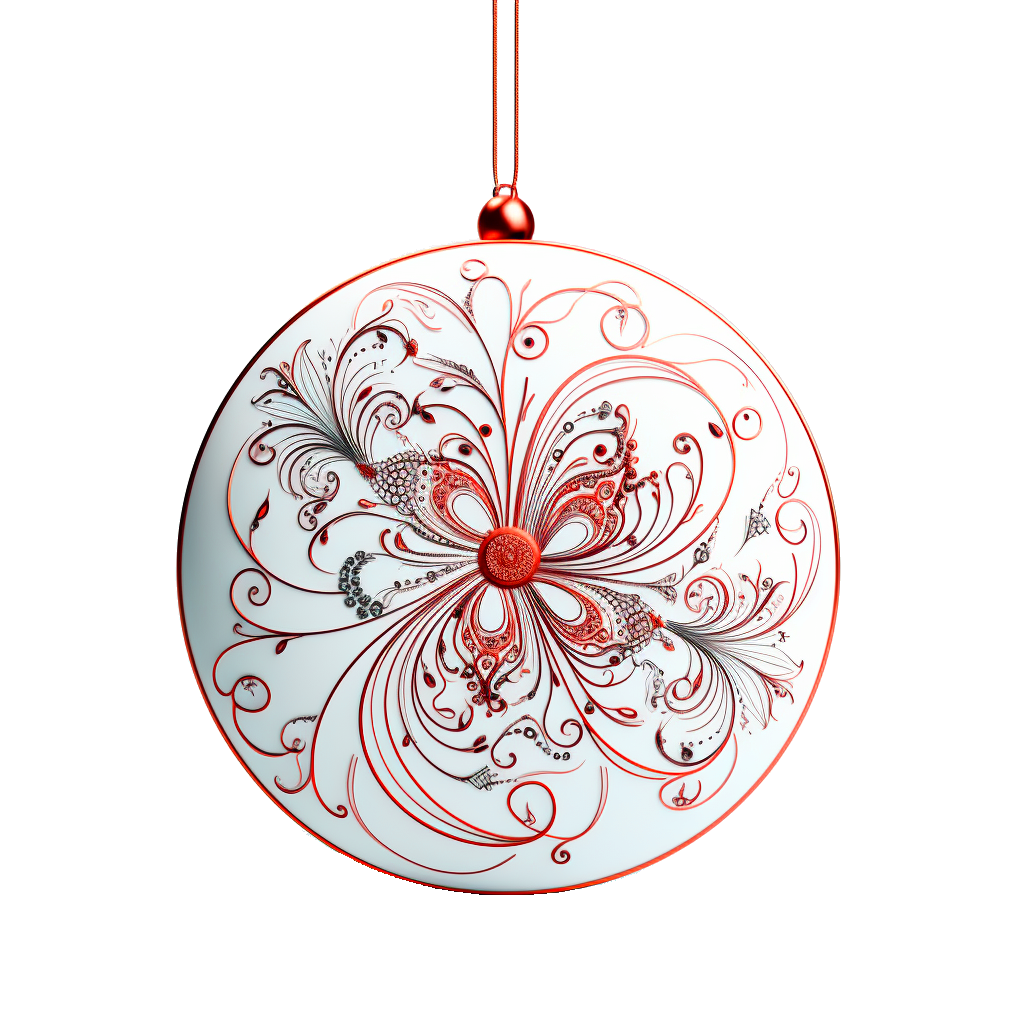
\includegraphics[width=0.3\linewidth]{08dimension2.png}		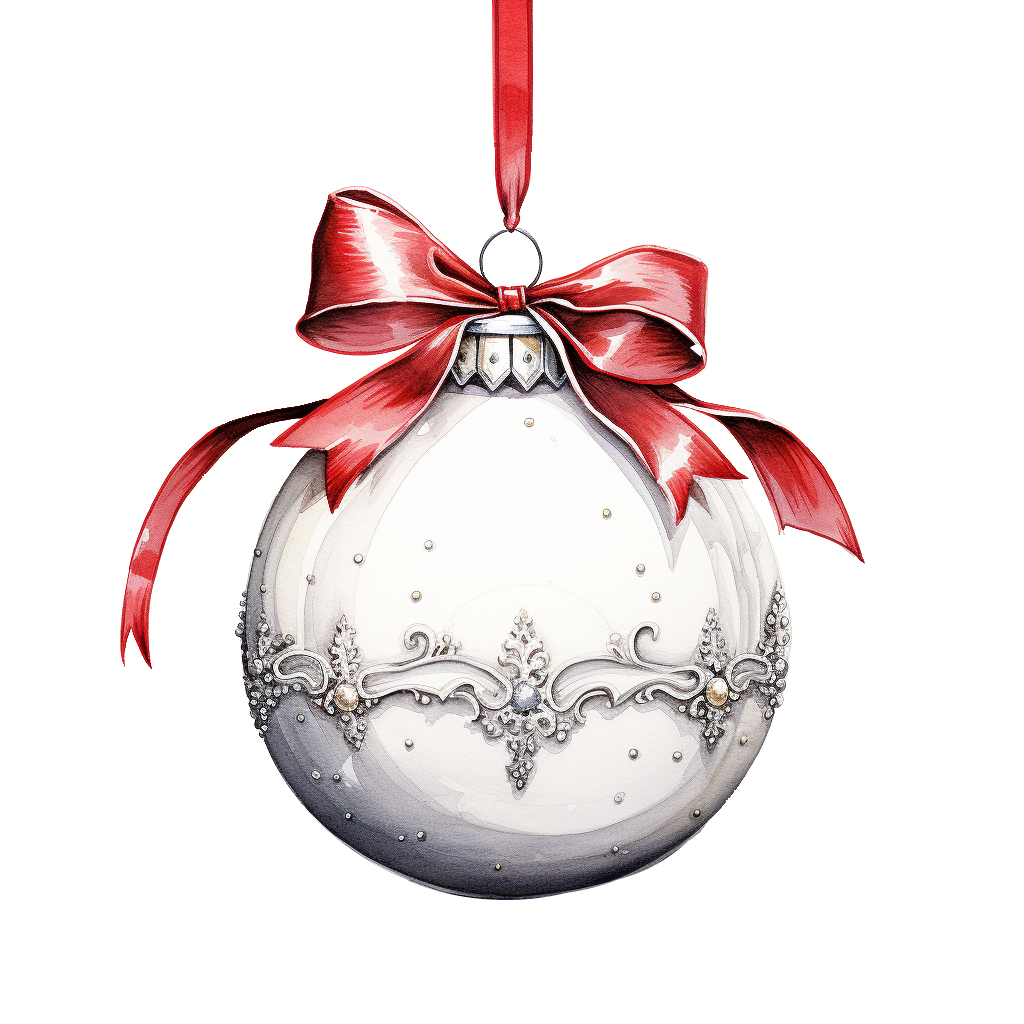
\includegraphics[width=0.3\linewidth]{08dimension3.png}
		
		Christmas decorations in 1,2 and 3 dimensions.
	\end{center}
	
	The volume of a $n$-dimensional ball of radius $R$ is given by: $\mathcal{V} = C_n R^n$.
	The constants $C_n$ follow the rule $C_n = \frac{2\pi}{n} \cdot C_{n-2}$.
	
	\vspace{3cm}
	
	\textbf{What is the highest value that $C_n$ takes?} Round it to $10^{-2}$.
	
	\vspace{1cm}
	
	\textit{If the answer is $\frac{123456}{10^5}$, then submit “$1.23$”.}
	
	\vspace{5\baselineskip}
	
	\textit{\underline{Bonus:} What is $\lim_{n \to +\infty} C_n$?}
	
	% n=1:  C_n = 2          ~ 2.00000...
	% n=2:  C_n = pi         ~ 3.14159...
	% n=3:  C_n = 4pi/3      ~ 4.18879...
	% n=4:  C_n = pi²/2      ~ 4.93480...
	% n=5:  C_n = 8pi²/15    ~ 5.26379... <<< largest !!!
	% n=6:  C_n = pi^3/6     ~ 5.16771...
	% n=7:  C_n = 16pi^3/105 ~ 4.72477...
	% n=8:  C_n = pi^4/24    ~ 4.05871...
	% n=9:  C_n = 32pi^4/945 ~ 3.29851...
	% n=10: C_n = pi^5/120   ~ 2.55016...
	% converges to 0 as n -> +00
	
\end{document}